\documentclass[a4paper,masters,en,listoffigures,listoftables]{NMBU}

% If you'd like to use chapters instead of sections, add 'book' to the options, as \documentclass[book,...]{NMBU}. Recall that you now have to use \chapter{} and then \section{}, \subsection{}, ... 

%\usepackage[nohyperlinks]{acronym} % If you need a List of Acronyms, consider using this package

% \usepackage[font=small]{caption} % if you prefer smaller captions
% \captionsetup{width=0.9\linewidth} 

% Word of advice: When you are done with your thesis, change the compiler in Overleaf to XeLaTeX! This will make your fonts and title page look much nicer than in pdfLaTeX. Just go to "Menu", in the "Settings", find "Compiler" and change to XeLaTeX.

% The NMBU style package is designed to help you write the cover and back page automatically. Make sure to include the information below to generate your title. You can set the language you are writing in with "en" for english, "bm" for bokmål, or "nn" for nynorsk.

% A table of contents is automatically included. If you have more than one figure, you need a list of figures by adding "listoffigures" to the documentclass parameters. If you have more than one table, you need a list of tables by adding "listoftables" to the documentclass parameters.

% Additional packages
\usepackage{algorithm}
\usepackage{algpseudocode}  % modern and recommended
\usepackage[intoc]{nomencl}
\makenomenclature

\renewcommand{\algorithmicrequire}{\textbf{Input:}}
\renewcommand{\algorithmicensure}{\textbf{Output:}}
\renewcommand{\v}[1]{\boldsymbol{#1}}

% If you would like to have a bibliography with named authors, organised alphabetically, add "namedauthors" to the parameters of the document class.
\addbibresource{bib.bib} % here you include the bibliography file. 
\graphicspath{{../figures/}}

% If you are using Norwegian dates in your bibliography, add "norwegiandates" to the document class.

% When you finish your thesis, switch the LaTeX compiler from pdfLaTeX to XelaTeX (on Overleaf, "Menu"->"Compiler"). This is for 2 reasons: 1) to produce your front page with the Arial font; 2) XeLaTeX produces better fonts and (usually) smaller PDFs. Every kilobyte of space we save helps reduce CO2 emissions :)

% Good luck with your thesis! If you get in trouble with LaTeX stuff, write to me: leonardo.rydin@gmail.com

% In your .tex file, you need to include the following information to produce the first page of your thesis

\title{Matrix-Free Randomized Sketching for Column-Norm Estimation of Discretized PDE Operator}
\author{Elias Jegervatn Severinsen}
\thesisyear{2026}
\credits{30}
\faculty{Faculty of Science and Technology}
\studyprogramme{Data Science}
\supervisor{Ole Løseth Elvetun, Jonas Kusch} % Include the name of the supervisor or supervisors (this is added to the metadata of the PDF)
%\engtitle{} % Only if you write a thesis in a Scandinavian language

% You should also use the "\abstract" and "\sammendrag" to produce those. If you are writing in a Scandinavian language, the sammendrag will appear first.
\abstract{This thesis uses randomized linear algebra for estimation of a discrete PDE operator.}
\sammendrag{Denne masteroppgaven bruker randomisert lineær algebra for mastrise-fri estimering av PDE-operatorer.}
%\acknowledgements{} You can add acknowledgements here. In Scandinavian languages, use "\foreword{}" (or if in English you prefer Foreword to Acknowledgements). The foreword comes before the abstract.

\begin{document}

% If you need a List of Acronyms, place them before the \startthesis command. You will need "\usepackage[nohyperlinks]{acronym}", see line 4.

%\section*{List of Symbols}
% \begin{acronym}
%   \acro{TSO}{Transmission System Operator}
%   \acro{LSTM}{Long Short-Term Memory}
%\end{acronym}

\section*{List of Symbols}

\begin{tabular}{ll}
    $\Omega$ & Problem domain \\
    $\partial\Omega$ & Domain boundary \\
    $A$ & Stiffness matrix \\
    $M$ & (Domain) mass matrix \\
    $M_{ds}$ & Boundary mass matrix \\
    $K$ & Discrete forward operator \\
    $K^*$ & Adjoint of the discrete forward operator \\
    $W$ & Weight matrix in the regularization \\
    $\lambda$ & Regularization parameter \\
    $\Xi$ & Random test matrix
\end{tabular}


\startthesis % This command will separate the Roman-numbered pages above and the Arabic-numbered pages below as well as create the table of contents, list of figures, list of tables, and potentially list of acronyms

\section{Introduction}

\clearpage
\section{Mathematical background}

\nomenclature{$\Omega$}{Computational domain}
\nomenclature{$\partial\Omega$}{Boundary of the domain}
\nomenclature{$A$}{Stiffness matrix}
\nomenclature{$M$}{Mass matrix}

\subsection{The forward operator}
\begin{figure}[htbp]
    \centering
    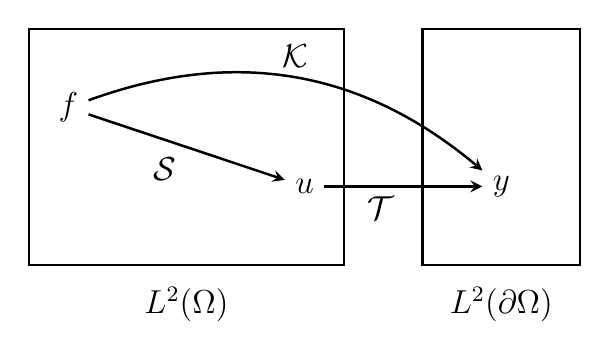
\begin{tikzpicture}[
        >=stealth,
        line width=0.9pt,
        every node/.style={font=\large}
    ]
    % Boxes
    \draw (0,0) rectangle (4,3);
    \draw (5,0) rectangle (7,3);
    
    % Space labels L^2
    \node at (2,-0.5) {$L^2(\Omega)$};
    \node at (6,-0.5) {$L^2(\partial\Omega)$};
    
    % f, u, and y points
    \node (f) at (0.5,2) {$f$};
    \node (u) at (3.5,1) {$u$};
    \node (y) at (6,1) {$y$};
    
    % Operator S
    \draw[->]
      (f) -- (u)
      node[midway, below left] {$\mathcal S$};
    
    % Operator T
    \draw[->]
      (u) -- (y)
      node[midway, below, xshift=-2.8mm] {$\mathcal T$};
    
    % Operator K
    \draw[->]
      (f) to[out=20, in=140]
      node[midway, above] {$\mathcal{K}$}
      (y);
    \end{tikzpicture}
    \caption{The forward operator $\mathcal K = \mathcal T \circ \mathcal S$ which maps $f$ to $y$.}
    \label{fig:forward_operator}
\end{figure}

Let $\Omega \subset \mathbb R^2$ be a bounded domain with boundary $\partial \Omega$. I consider the following second-oder elliptic boundary value problem (BVP):
\begin{eqnarray}\label{eq:pde}
    \begin{aligned}
    -\nabla \cdot \sigma\nabla u + ku &= f \quad \text{in } \Omega, \\
    \frac{\partial u}{\partial \v n} &= 0 \quad \text{on } \partial\Omega,
    \end{aligned}
\end{eqnarray}
where $k > 0$ and $\sigma, f \in H^1(\Omega)$ (TODO: hva er $\sigma$). This is a diffusion-reaction equation with Neumann boundary conditions. Equation~\eqref{eq:pde} defines a mapping $\mathcal S: H^1(\Omega) \rightarrow H^1(\Omega)$. If $f \in H^1(\Omega)$ is the source function (the input), then Equation~\eqref{eq:pde} maps $f$ to $\mathcal S f = u$ (the output). 

Introduce the trace operator $\mathcal T: H^1(\Omega) \rightarrow H^1(\partial\Omega)$, defined by
\begin{equation}\label{eq:trace}
    \mathcal T: u \mapsto g = u|_{\partial\Omega}.
\end{equation}
$\mathcal T u$ represents the observed values of $u$ on the boundary of $\Omega$. Operator~\eqref{eq:pde} and \eqref{eq:trace} defines the forward operator $\mathcal K: H^1(\Omega) \rightarrow H^1(\partial\Omega)$, 
\begin{equation}
    \mathcal K = \mathcal T \circ \mathcal S,
\end{equation}
which is a mapping from the source function $f$ to the observed output $g = \mathcal K f$ on the boundary $\partial \Omega$. Figure~\ref{fig:forward_operator} illustrates the components of the forward operator, which defines the inverse problem: given observed boundary function $g$, we seek a source function $f$ such that $\mathcal{K} f = g$. In order to solve such a problem computationally, the problem must be discretized. This is done through the finite element method, described in the following sections.


\subsection{The variational formulation}
To derive a finite element formulation of Eq.~\eqref{eq:pde} and the forward operator $\mathcal K$, I first reformulate the boundary value problem in its variational (weak) from. Multiplying the differential equation by a test function $v \in H^1(\Omega)$, integrating over $\Omega$, and applying Green's identity and the Neumann boundary conditions, results in the following variational formulation: find $u \in H^1(\Omega)$ such that
\begin{equation}\label{eq:variational_formulation}
    \int_{\Omega} (\sigma \nabla u \cdot \nabla v + k u v) \, dx = \int_{\Omega} f v \space \, dx,
    \text{ for all } v \in H^1(\Omega).
\end{equation}
For further details, see Section~4 in Larson and Bengzon \cite{larson_finite_2013}.


\subsection{The finite element method}
\begin{figure}[htbp]
    \centering
    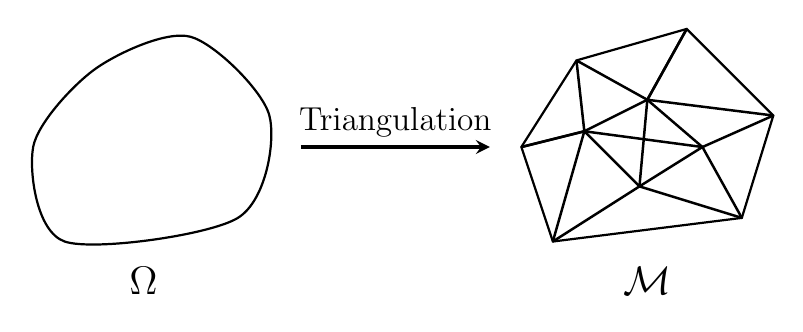
\begin{tikzpicture}[
        >=stealth,
        line width=0.9pt,
        every node/.style={font=\large}
    ]
    % Left: continuous domain Omega
    \begin{scope}[shift={(0,0)}]
      % Draw a smooth-ish domain
      \draw[thick]
        plot [smooth cycle, tension=0.5]
        coordinates {
          (0,0)
          (2.2,0.3)
          (2.6,1.6)
          (1.6,2.6)
          (0.4,2.2)
          (-0.4,1.2)
        };
      % Label
      \node at (1,-0.5) {\Large $\Omega$};
    \end{scope}
    
    % Middle arrow
    \begin{scope}[shift={(4.2,1.2)}]
        \draw[very thick,->] (-1.2,0) -- (1.2,0);
        \node[above] at (0,0) {Triangulation};
    \end{scope}
    
    % Right: triangulated mesh M
    \begin{scope}[shift={(6.2,0)}]
        % Outer polygon (approximation of Omega)
        \coordinate (A) at (0,0);
        \coordinate (B) at (2.4,0.3);
        \coordinate (C) at (2.8,1.6);
        \coordinate (D) at (1.7,2.7);
        \coordinate (E) at (0.3,2.3);
        \coordinate (F) at (-0.4,1.2);
        % Boundary
        \draw[thick] (A)--(B)--(C)--(D)--(E)--(F)--cycle;
        % Some interior points
        \coordinate (P1) at (1.1,0.7);
        \coordinate (P2) at (1.9,1.2);
        \coordinate (P3) at (1.2,1.8);
        \coordinate (P4) at (0.4,1.4);
        % Draw triangulation
        \draw (A)--(P1)--(B);
        \draw (B)--(P2)--(C);
        \draw (C)--(P3)--(D);
        \draw (D)--(P3)--(E);
        \draw (E)--(P4)--(F);
        \draw (F)--(P4)--(A);
        \draw (P1)--(P2)--(P3)--(P4)--cycle;
        \draw (P1)--(P3);
        \draw (P2)--(P4);
        % Label
        \node at (1.2,-0.5) {\Large $\mathcal M$};
    \end{scope}
    \end{tikzpicture}
    \caption{The triangulation $\mathcal{M}$ (the mesh) of $\Omega$. $\mathcal{M}$ is made up of $N$ nodes located at the vertices (corners) of the triangles.}
    \label{fig:triangulation}
\end{figure}
Let $\mathcal M$ be a triangulation of $\Omega$ made up of $N$ nodes, with $N_b$ boundary nodes, see Fig.~\ref{fig:triangulation} as an example. The finite element space is the finite-dimensional $V_h \subset H^1(\Omega)$,
\begin{equation}\label{eq:fem_space}
    V_h = \{v \in C^0(\Omega) : v|_M \text{ is linear for all } M \in \mathcal M \}.
\end{equation}
This is the space of all continuous functions which are piecewise linear on $\mathcal{M}$. Let $\Phi = \{\phi_1, \dots, \phi_N\}$ be a basis $V_h$, i.e., $\operatorname{span}(\Phi) = V_h$. The basis functions $\phi_1, \dots, \phi_N$ are typically hat functions (see \parencite[p.~51]{larson_finite_2013}). For each node making up the mesh $\mathcal{M}$, there is a corresponding basis function. Since the mesh $\mathcal{M}$ consists of $N$ nodes and $N_b$ boundary nodes, then the basis set $\Phi$ must contain $N$ basis function, with $N_b$ being located on the mesh boundary.

By replacing $H^1(\Omega)$ with $V_h$ in Eq.~\eqref{eq:variational_formulation}, I get the finite element method: find $u_h \in V_h$ such that
 \begin{equation}\label{eq:fem_formulation}
    \int_{\Omega} (\sigma \nabla u_h \cdot \nabla v + k u_h v) \, dx = \int_{\Omega} f v \space \, dx,
    \text{ for all } v \in V_h.
\end{equation}


\subsection{The discrete inverse problem}
In order to represent the forward operator $\mathcal{K} = \mathcal{T} \circ \mathcal{S}$ in a discrete form which can be represented computationally, both the PDE operator $\mathcal S$ and the trace $\mathcal T$ must be discretized, i.e., their matrix representations $S$ and $T$ must be found. Using finite element representations of $f$, $u$ and $g$, the problem $\mathcal{K}f = g$ can be expressed in terms of a system of linear equations.

Discretizing the PDE operator $\mathcal{S}$, which represents the finite element formulation in Eq.~\eqref{eq:fem_formulation}, is done by replacing the source function $f$ by its finite element approximation $f_h \in V_h$. Since both $u_h$ and $f_h$ are functions of the subspace $V_h$, they may be written as a linear combinations of the basis functions $\phi_1, \dots, \phi_N$,
\begin{equation}\label{eq:uh_and_fh}
    u_h = \sum_{j=1}^{N} u_j \phi_j, \quad
    f_h = \sum_{j=1}^{N} x_j \phi_j.
\end{equation}
where $\{ \phi_1, \dots, \phi_N \}$ is a basis for $V_h$. Let $\v x = [x_1, \, \dots, \, x_N]$ and $\v u = [u_1, \, \dots, \, u_N]$ be the coefficient vectors for $f_h$ and $u_h$, respectively.
By inserting Eq.~\eqref{eq:uh_and_fh} into the finite element formulation in Eq.~\eqref{eq:fem_formulation}, following system of linear equations (matrix-vector equation) is obtained:
\begin{equation}\label{eq:matrix_vector_equation}
    A \v x = M \v u.
\end{equation}
$A$ is known as the stiffness matrix and $M$ the mass matrix. Solving Eq.~\eqref{eq:matrix_vector_equation} for $\v x$, we get that $\v x = A^{-1} M \v u$, so the discretization $S\in \mathbb{R}^{N \times N}$ of the PDE operator $\mathcal S$ is therefore
\begin{equation}\label{eq:discrete_S}
    S = A^{-1}M.
\end{equation}
Note that $S$ maps the coefficients $\v x$ of $f_h$ to the coefficients $\v u$ of $u_h$ in their finite element representations given in Eq.~\eqref{eq:uh_and_fh}.

The discretization $T: \mathbb{R}^N \rightarrow \mathbb{R}^{N_b}$ of $\mathcal T$ is a $N_b \times N$ matrix which extracts the boundary coefficients of a function. Each row has one element equal to 1, corresponding to the boundary node index, and 0s elsewhere. Next, using the discrete operators $S$ and $T$, we get that the discretized formulation of the forward operator $\mathcal K = \mathcal T \circ \mathcal S$ is
\begin{equation}\label{eq:discrete_K}
    K = T S = T A^{-1} M \in \mathbb R^{N_b \times N}.
\end{equation}

By denoting the boundary coefficients of $\v u$ by $\v y$, i.e., $T \v u = \v y$, we can formulate $\mathcal{K}f = u|_{\partial\Omega}$ in its discretized version:
\begin{equation}\label{eq:inverse_problem}
    K \v x = \v y.
\end{equation}
Equation~\eqref{eq:inverse_problem} represents the discrete inverse problem: given observed boundary data $\v y$, we seek the coefficient vector $\v x$ of the source term $f_h$.

%In practice, this system is often **ill-posed** due to the large null space of $K$ and the accumulation of numerical errors in $A^{-1}$. As a result, naive solutions of Eq.~\eqref{eq:inverse_problem} are highly sensitive to noise in $\v y$, motivating the need for regularization techniques. In the following section, we discuss classical Tikhonov regularization and introduce the weighted approach that will be explored in this thesis.


\subsection{Tikhonov regularization}
Theory on Tikhonov regularization,
\begin{equation}
    \min_{x \in \mathbb R^n} \| A x - b \|^2 + \lambda^2 \| x \|^2
\end{equation}


\subsection{Randomized SVD}
\begin{figure}[thbp]
    \centering
    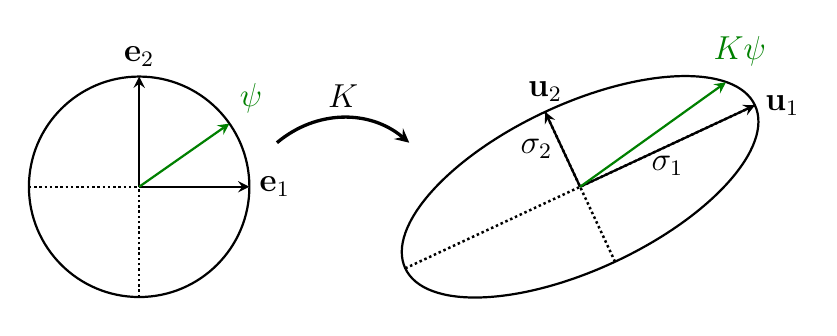
\begin{tikzpicture}[
        scale=0.7,
        >=stealth,
        line width=0.9pt,
        every node/.style={font=\large}
    ]
    % Left: unit circle
    \begin{scope}[shift={(0,0)}]
      % circle
      \draw[thick] (0,0) circle (2);
      % dotted guidelines
      \draw[densely dotted] (-2,0) -- (0,0);
      \draw[densely dotted] (0,-2) -- (0,0);
      % e1, e2
      \draw[thick,->] (0,0) -- (2,0) node[right] {$\mathbf e_1$};
      \draw[thick,->] (0,0) -- (0,2) node[above] {$\mathbf e_2$};
      % omega, length=2, angle=35
      \draw[thick,->,Green] (0,0) -- ({2*cos(35)},{2*sin(35)}) node[above right] {$\boldsymbol{\psi}$};
    \end{scope}
    
    % Middle: K arrow
    \begin{scope}[shift={(3.5,0)}]
      \draw[very thick,->]
        (-1,0.8) to[out=40, in=140] (1.4,0.8);
      \node[above] at (0.2,1.25) {$K$};
    \end{scope}
    
    % Right: ellipse + vectors
    \begin{scope}[shift={(8,0)}, rotate=25]
      % ellipse
      \draw[thick] (0,0) ellipse (3.5 and 1.5);
      % dotted principal axes
      \draw[densely dotted] (-3.5,0) -- (3.5,0);
      \draw[densely dotted] (0,-1.5) -- (0,1.5);
      % u1 and u2
      \draw[thick,->] (0,0) -- (3.5,0)
        node[midway, below] {$\sigma_1$}
        node[right] {$\mathbf u_1$};
      \draw[thick,->] (0,0) -- (0,1.5)
        node[midway, left] {$\sigma_2$}
        node[above] {$\mathbf u_2$};
      % omega
      \draw[thick,->,Green] (0,0) -- (3.2,0.6)
      node[above, xshift=5pt, yshift=2pt] {$K\boldsymbol{\psi}$};
    \end{scope}
    \end{tikzpicture}
    \caption{The geometry of the rSVD. A random sample $K\v\psi$ aligns mostly with the first left singular value. The illustration is inspired by Fig.~9.1 in Tropp \cite{tropp_acm_2021}.}
    \label{fig:rsvd}
\end{figure}
The rSVD is a technique used to compute a rank-$k$ approximation of an $m\times n$ matrix without computing the SVD. The core idea is to use random sampling to find a low-rank matrix $Q$ which approximates the range of $A$, project $A$ onto $\operatorname{span}(Q)$, and compute the SVD of the projection. The projection $B=Q^TA$ will, with high probability, capture the dominant actions of $A$, and the SVD of $B$ will yield a good approximation \cite{halko_finding_2011}. This procedure is summarized in Algorithm \ref{alg:rsvd}. The construction of an orthonormal basis $Q$ of $Y$ is done through a QR factorization. Note that the approximation $A\approx QQ^T A$ and the approximate factorization $A\approx U\Sigma V^T$ produced by rSVD have the same error. This can be seen by observing that $QQ^TA = QB = Q\tilde U\Sigma V^T$, and setting $U=Q\tilde U$.
\begin{algorithm}[!htbp]
\caption{rSVD}
\label{alg:rsvd}
\begin{algorithmic}[1]
    \Require $A\in\mathbb R^{m\times n}$, target rank $k$, oversampling parameter $p$.
    \Ensure Approximate rank-$k$ factorization $U\Sigma V^T$.
    \State Generate a random $n\times(k+p)$ test matrix $\Omega$.
    \State Compute $Y = A\Omega$.
    \State Form an orthonormal basis $Q$ of $Y$.
    \State Set $B = Q^TA$.
    \State Compute the SVD $B = \tilde U\Sigma V^T$.
    \State Set $U = Q\tilde U$. 
\end{algorithmic}
\end{algorithm}


\subsection{Tips}
When you are closely following a book to explain something, which is often the case in a theory section, you can write at the start of the section you are about to introduce: ``This section follows closely the reference book by Sumiyoshi Abe and Yuko Okamoto, \emph{Nonextensive Statistical Mechanics and Its Applications}~\parencite[p.~32]{Abe2001nonextensive}.''

A Master's~\cite{LastName2045norwegian} or a PhD thesis~\cite{Temult2038binding} should include the name of the university wherein it was written, as well as the year. Moreover, it should include a URL to the work, when available.

\clearpage
\section{Methods}
\begin{figure*}[thbp]
    \centerline{\includegraphics[width=\textwidth]{S_and_T_example.png}}
    \caption{Example of the discrete forward operator $u|_{\partial\Omega} = T u = T S f$. Left: the source function $f$. Middle: the full output $u$. Right: the observed output $u|_{\partial\Omega}$ of $u$ on the boundary of $\Omega$.}
    \label{fig:S_and_T_example}
\end{figure*}

\begin{algorithm}[!htbp]
\caption{Discrete Operator rSVD Approximation of $K$}
\label{alg:discrete_rsvd}
\begin{algorithmic}[1]
    \Require Forward operator $K: \mathbb{R}^N \to \mathbb{R}^{N_b}$, adjoint operator $K^*: \mathbb{R}^{N_b} \to \mathbb{R}^N$, mass matrices $M_{dx}, M_{ds}$, target rank $p$
    \Ensure Approximate rank-$p$ factorization $K \approx U \Sigma V^T$
    
    \State \textbf{Range sketch:}
    \For{$i = 1, \dots, p$}
        \State Draw a random vector $\v \xi_i \in \mathbb{R}^N$
        \State Apply the forward operator: $\v y_i = K \v \xi_i \in \mathbb{R}^{N_b}$
    \EndFor

    \State Form the matrix $Y = [\v y_1, \dots, \v y_p] \in \mathbb{R}^{N_b \times p}$ \Comment{Equivalent to $Y = K \Xi$}
    \State Compute an orthonormal basis: $Q = \text{orth}(Y)$

    \State \textbf{Projection onto the basis:}
    \For{$i = 1, \dots, p$}
        \State Let $\v q_i$ be the $i$-th column of $Q$
        \State Compute $\tilde{\v{q}}_i = M_{ds}^{-1} \v{q}_i$
        \State Set $\v{b}_{\text{adj},i} = K^* \tilde{\v{q}}_i$
        \State Let $\v{b}_i = b_{\text{adj},i}^T M_{dx}$ \Comment{$i$-th row of $B$}
    \EndFor
    \State Form the projected matrix $B = \begin{bmatrix} b_1 \\ \vdots \\ b_p \end{bmatrix} \in \mathbb{R}^{p \times N}$ \Comment{Equivalent to $B = Q^T Y$}

    \State Compute the SVD: $B = \tilde U \Sigma V^T$
    \State Set $U = Q \tilde U$
    
\end{algorithmic}
\end{algorithm}



\clearpage
\section{Literature Review}


\clearpage
\section{Methodology}
In the methodology, you might include mentions of various \texttt{python} (or other programming languages) packages.


\clearpage
\section{Results}


\clearpage
\section{Discussion}

\clearpage
\section{Conclusion}

% Note that the appendices should come after the bibliography, not before.
\clearpage
\references % This command prints out your bibliography

\clearpage
\appendices % This command is needed to start the appendix section and number the figures and tables accordingly. You should still use "\section"s to make your appendices.

\end{document}
